\chapter{Introduction}\label{Motivation}
%
\epigraph{\textit{I wish to God these calculations had been executed by steam.}}{Charles Babbage}
The advent of the modern digital computer, as formalised by Alan Turing,\cite{Turing1937} ignited the field of computational physics, aided by preexisting theoretical formulations of algorithms. Starting from the first experiments with Monte Carlo (MC) simulations in the 1930s by Fermi and the formulation of the Markov-Chain Monte Carlo (MCMC) technique by Ulam in the 1940s, von Neumann programmed the 18,000 vacuum-tube Electronic Numerical Integrator and Computer (ENIAC) computer to investigate neutron diffusion in fissionable materials.\cite{metropolis1987beginning} This success paved the way for the integration of Newton's equations of motion to compute the time evolution of a many-body system.\\

%\subsection{Fermi–Pasta–Ulam–Tsingou problem}
In 1953, Fermi, Pasta, Ulam and Tsingou simulated a 1-dimensional analogue of atoms in a crystal, formed of masses connected by springs that obey Hooke's law and a weak non-linear term on the Mathematical Analyzer Numerical Integrator and Automatic Computer Model I (MANIAC I) computer. Using this, they were able to simulate the time evolution of the energy of a system to understand the origins of irreversibility in nature. This is known as the Fermi–Pasta–Ulam–Tsingou problem.\cite{fermi1955studies}\\

%\subsection{Alder-Wainwright}
The first use of molecular dynamics (MD) simulations were implemented by Alder and Wainwright in 1957 using an IBM 704 computer, where they simulated the elastic collisions in a hard sphere fluid composed of a maximum of 108 particles. They outlined the importance of the evolution in time of a system towards a steady-state, which was outside the scope of the preexisting MC techniques and within the grasp of MD. Conscious of the limitations of computational power that was available, they acknowledge that their work is qualitative and indicate that, given better resources, simulations could give quantitative statistical averages of thermodynamic properties at equilibrium. Unlike modern implementations of MD with continuous potentials, Alder and Wainwright modelled their hard sphere liquid using discontinuous potentials where events such as particle collisions define the simulation statistics.\cite{Alder1959}\\

%\subsection{Rahman (liquid argon)}
Arguably the first MD simulations that reflected the verifiability of the method as a science, by comparing with experiment, are those of liquid argon by Rahman in 1964 using a Control Data Corporation (CDC) 3600 computer. Similar to modern uses of MD, Rahman's simulations modelled the interactions using a pairwise Lennard-Jones potential, first proposed in 1932,\cite{lennard1932processes} of an 864 particle system. Using these MD simulations, a radial distribution function and the self-diffusion constant were calculated to compare to experiment, where the latter was found to be within 15\% of the experimental value. The discrepancy between predicted observables and experiments were in the range of 20\%, which spurred Rahman to tweak the repulsive part of the Lennard-Jones potential; forcefield development therefore reared its head as soon as MD came to fruition.\cite{rahman1964correlations}\\

The highlight of the history of molecular simulations is undoubtedly the 2013 Nobel Prize in Chemistry for the development of multiscale models for complex chemical systems. It recognised the pioneering work of Martin Karplus, Michael Levitt and Arieh Warshel in a range of molecular simulation techniques, from quantum chemistry to MD simulations of biomolecules. Most notable among them is the development of the hybrid quantum mechanics/molecular mechanics (QM/MM) simulation technique by Levitt and Warshel.\cite{warshel1976theoretical} This method \edit{combined} the accuracy of quantum mechanical calculations with the efficiency of \edit{MD} simulations by defining a QM region within an encompassing MM region. In another seminal work, they studied the folding of a model bovine pancreatic trypsin inhibitor protein in 1975, by simplifying the structure of the protein and simulating the system at $T=1000$\ K, to crudely solve for the global minimum through simulated annealing. This paper could be considered the first MD simulation of a biological process, albeit a simplified one.\cite{levitt1975computer} Of his many accomplishments, Martin Karplus and his group created the Chemistry at Harvard Macromolecular Mechanics (CHARMM) MD engine and coordinated its development, as well as formalising and parameterising various iterations of the CHARMM forcefield, which has been one of the primary forcefields used for simulating biological molecules.\cite{schmidt1993molecular} Karplus proposed the idea of first principles (\textit{ab initio}) molecular dynamics (AIMD) simulations in 1973, where trajectories would describe dynamic organic reactions as in MD, but be defined by quantum mechanical forces instead of semi-empirical mechanical techniques.\cite{wang1973dyanmics} 

\section{Current state-of-the-art in biomolecular simulations} \label{sec:sota_bio_sims}
\subsection{Groundbreaking simulations}

%\subsubsection{Big ones}
In 2006, MD simulations of an all-atom complete satellite tobacco mosaic virus (Fig.~\ref{fig:STMV}), in a system composed of a million particles, were conducted using the Nanoscale Molecular Dynamics (NAMD) MD engine for 50 ns. This work demonstrated the capacity for MD to study temporal properties of matter at such a large scale, which is at the heart of the mechanistic understanding of life itself. One of the major findings in this study was the conditional stability of the viral capsid \edit{i}n the presence of the enclosed ribonucleic acid (RNA).\cite{freddolino2006molecular} This was a profound result both from an evolutionary perspective and a computational one; to reveal the power of pairwise interaction parameters and a handful of algorithms, to describe the physio-chemical drivers at the heart of the function of biomolecular processes. 

\begin{figure}[H]
    \centering
    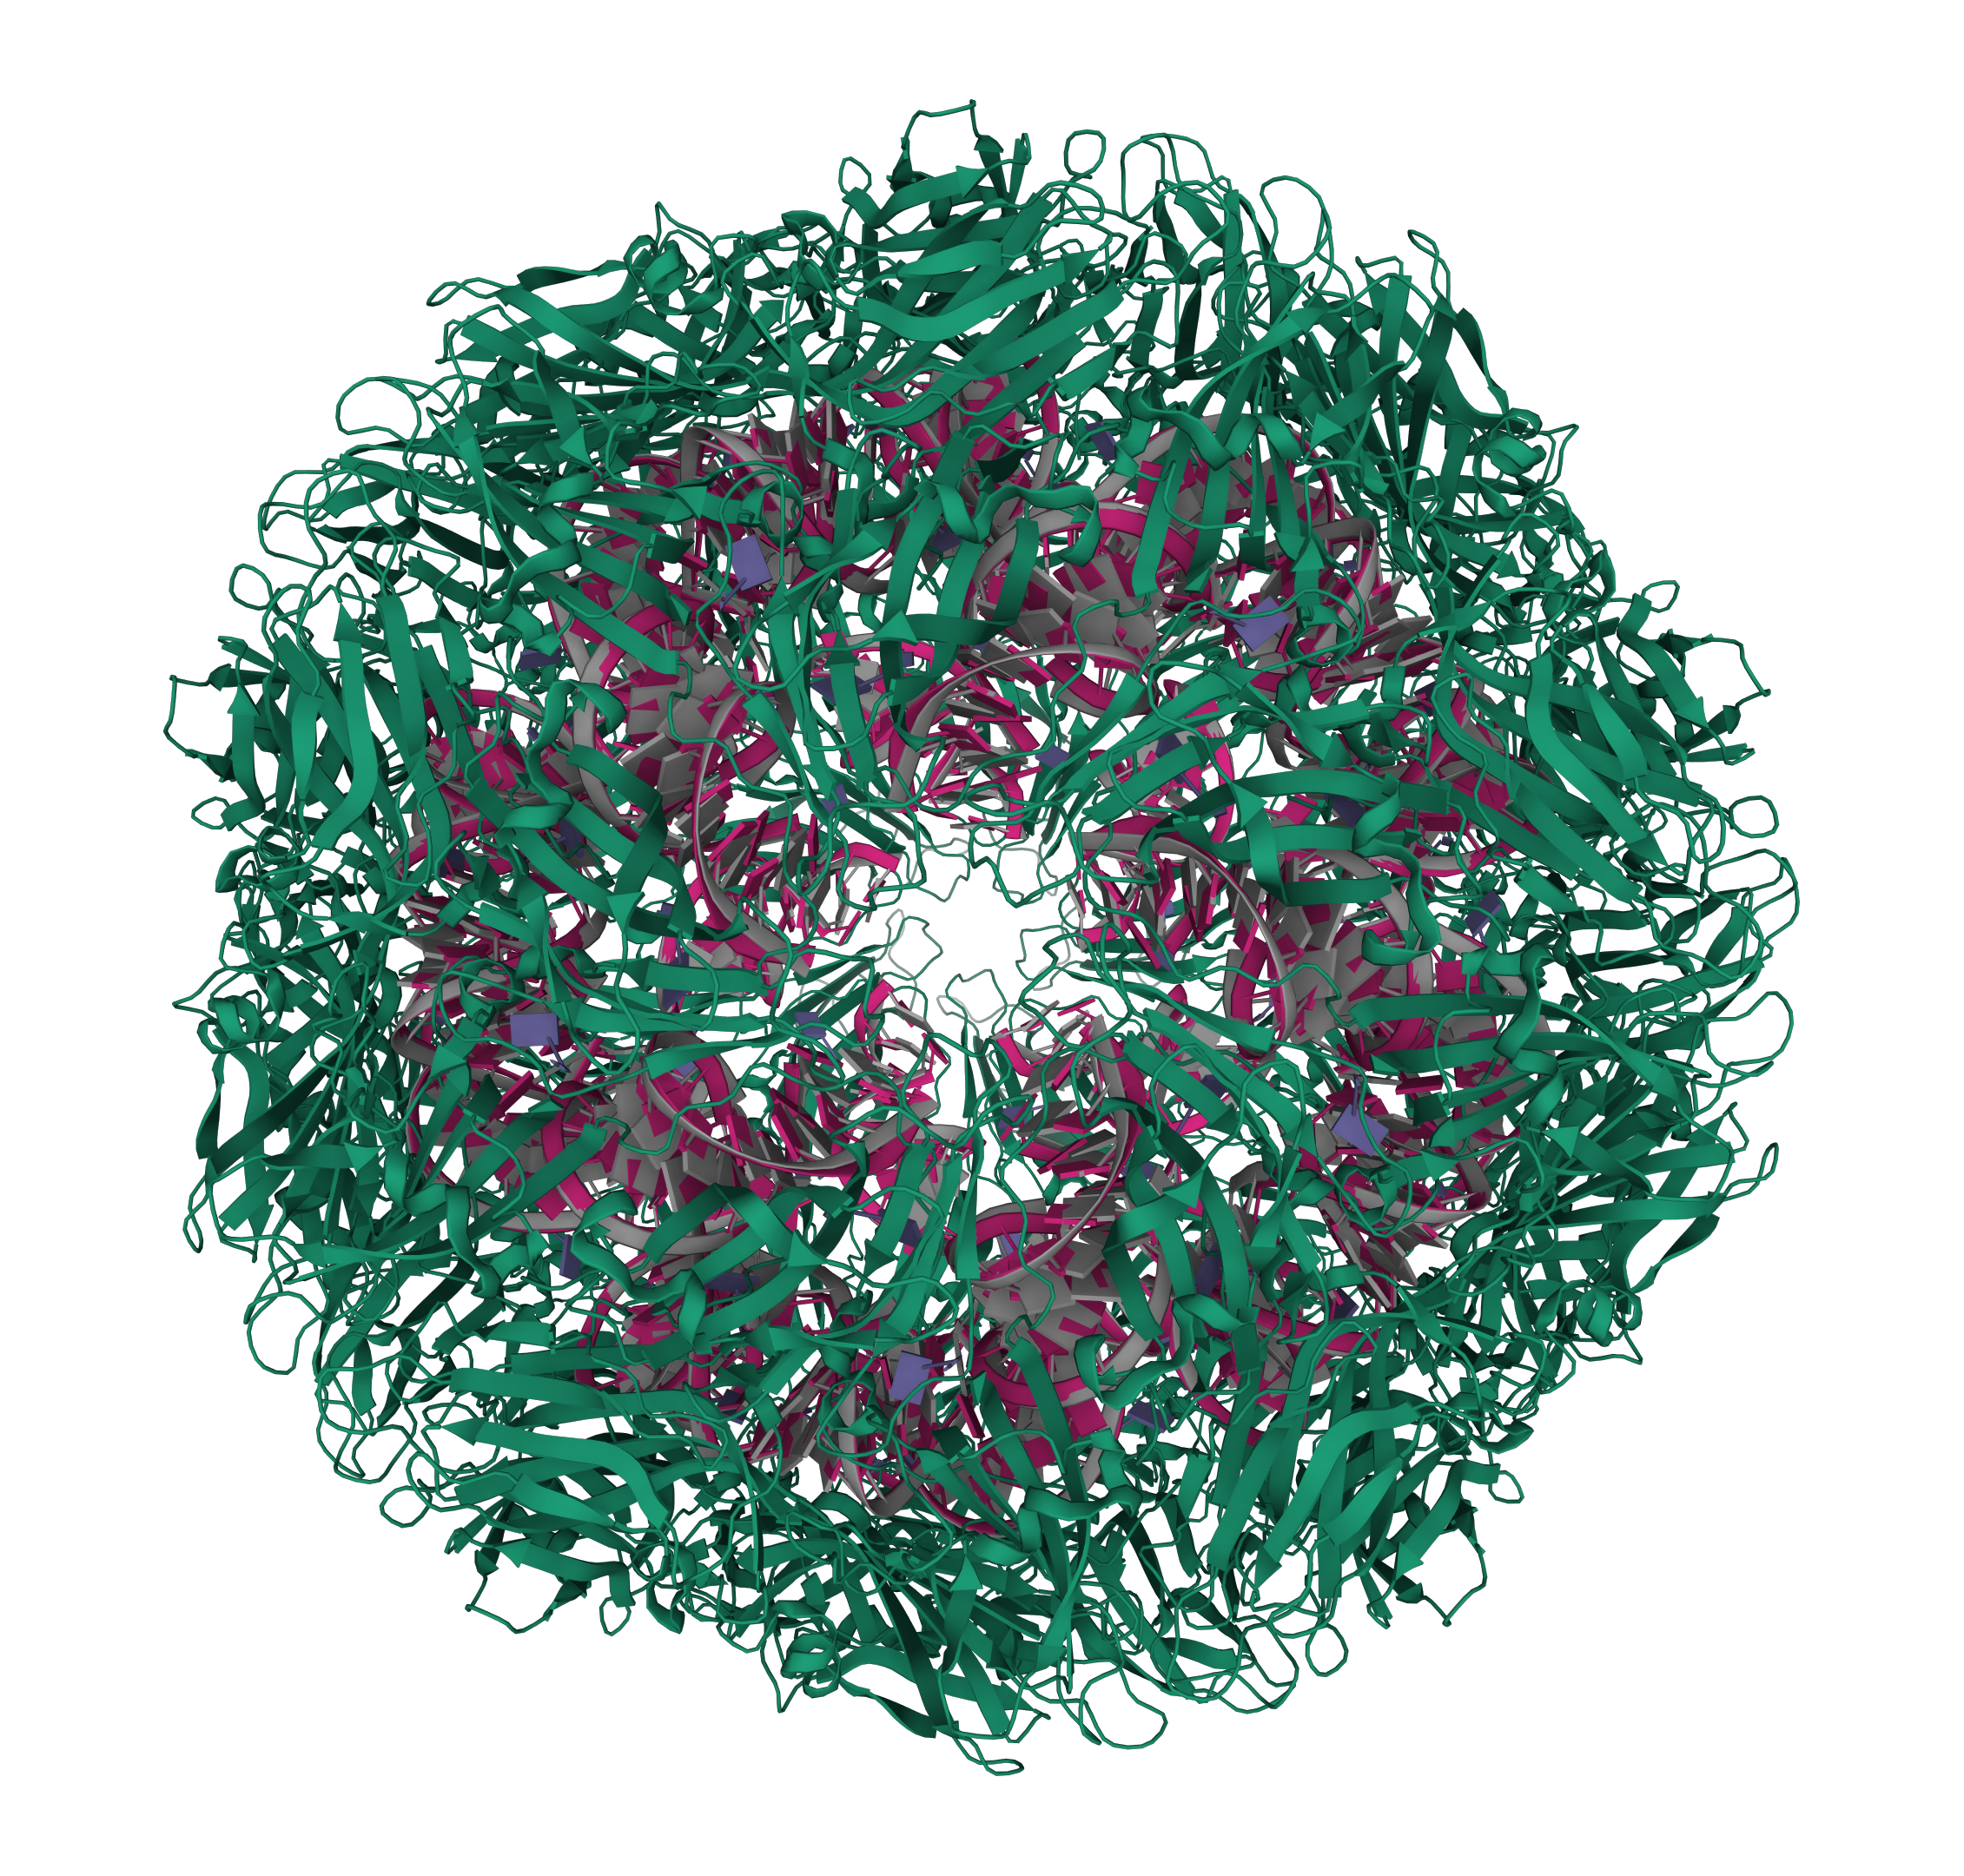
\includegraphics[width=0.7\textwidth]{figures/4OQ9.png}
    \caption{The structure of the satellite tobacco mosaic virus (PDB code 4OQ9), showing the protein capsid (green) enveloping the RNA (purple).\cite{Larson2014}}
    \label{fig:STMV}
\end{figure}
%
Using MD as a tool to investigate the structure and dynamics of systems out of the reach of conventional experimental methods, is therefore an avenue to advancing our understanding of biomolecular processes at the atomic scale. In the understanding of disease, an early breakthrough of MD-guided drug discovery is due to Andrew McCammon and colleagues. In their work, they performed 2 ns MD simulations of HIV integrase where they identified a cryptic trench which became a target for the first FDA approved HIV integrase inhibitor (raltegravir).\cite{schames2004discovery} \\

More recently the distributed computing project known as Fold@Home, originally set up by Vijay Pande in 2000, achieved exascale computing using a million personal computers from volunteers worldwide. Using this wealth of computational power, a plethora of MD simulations of protein dynamics were run to develop new therapeutics for a variety of diseases. A highlight of this effort came from the ongoing COVID-19 pandemic. The Fold@Home team ran a 0.1 second MD simulation to study the conformational changes in the SARS-CoV-2 spike protein to understand its role in evading an immune response, and similar to the example of HIV integrase, revealed cryptic binding sites for druggability.\cite{Zimmerman2020} \\

\subsection{Bespoke forcefield parametrisation} \label{sec:ff_devel}
Karplus' proposition to perform MD using QM forces, when correctly implemented, could circumvent the inherent inaccuracies of MD using generalised forcefields and be close to an exact MD. As an approach, AIMD is open to implementing any electronic structure theory method to calculate the atomic forces on-the-fly. The use of density functional theory (DFT) as a basis for calculating coupled electron-ion dynamics for AIMD was actualised by Car and Parrinello in 1985, resulting in a method known as Car-Parrinello MD (CPMD).\cite{Car1985} \\

This golden standard is --- in its modern form --- the closest we have come to accurately investigating the dynamics of matter at that scale. It is scale that also defines its limitations; AIMD simulations are restricted to system sizes and simulation times much smaller than the timescales at which important biomolecular processes such as protein conformational changes, ligand binding events and macromolecular interactions take place. Alternatively, more accurate forcefields may be an avenue to achieving a similar level of accuracy as in AIMD, and therefore provide the desired understanding of biology at the atomistic scale (see Chapter \ref{chapter:MD}). For decades, the parametrisation of forcefields has achieved wide coverage through extrapolating parameters from small molecular systems, and where necessary, optimised through experimental observables when a forcefield underperforms.\cite{Siu2012} The ability to reproduce the chemical properties of systems is hinged on whether the forcefield training and test sets include corresponding molecules. In the absence of rigorous testing, which is time consuming and certainly not a formal requisite to an MD investigation, the validity of predicted observables is certainly not guaranteed. The advantage of a large international MD community is the rapid identification of errors and the subsequent continuous integration of corrections by the forcefield developers. Importantly however, the persisting divergence from accuracy is almost exclusively limited to molecular systems with exotic chemistries.

\subsubsection{OpenFF initiative}
Accurate MD modelling has commercial potential with significant uptake by the pharmaceutical industry, in the form of the OPLS-3 forcefield,\cite{harder2016opls3} made exclusive to the D. E. Shaw Research (DESRES) developed Desmond MD engine.\cite{bowers2006scalable} In contrast, the Open Force Field (OpenFF) initiative is an open-source, collaborative and community-led project for the development of better forcefields.\cite{Qiu2020} OpenFF is parametrised using the ForceBalance forcefield optimisation software tool,\cite{wang2013systematic} which uses experimental and/or quantum mechanical calculations as reference data to produce forcefield parameters. With sufficient community-contributed data and a strong automated infrastructure, held together by good software development, the OpenFF Parsley forcefield aims to incorporate diverse chemistries for small molecules, and hence improve the accuracy of MD simulations within that niche. Parsley has achieved a similar accuracy for liquid properties when compared to other forcefields, such as the General Amber Force Field (GAFF), while showing improvements in the optimised geometries and conformational energetics of small molecules outside its training set.\cite{Qiu2020} However, it will not rival generalised forcefields on accuracy and wide coverage without the continued integration of data. The uptake of the forcefield may be somewhat retarded by the SMIRKS \cite{SMIRKS} \edit{N}ative Open Force Field (SMIRNOFF) parameter assignment formalism, which unlike general commonly applied forcefields is based on chemical perception, \edit{where the assignment of forcefield parameters is solely based on whether a bond between atoms is a single, double, triple or aromatic bond. This is unlike the assignment of complex atom type labels given to each atom to determine its interaction parameters with other atom types in conventional forcefield formats. The SMIRNOFF formalism is} not currently transferable to all MD engines. 

\subsubsection{Gaussian process regression}
Other groups have approached the forcefield question from a purely quantum mechanical perspective by learning a non-parametric tabulated forcefield of a system through the use of Gaussian process regression.\cite{zeni2018building, bartok2010gaussian, Vandermause2020} Such kernel based approaches set out to learn a local configuration relative to each atom in a system and the forces that act upon them from \textit{ab initio} methods such as DFT, on-the-fly. The accuracy of the resulting Gaussian process regression forcefield is determined by its ability to reproduce DFT forces. Gaussian process regression methods for forcefield development have so far been applied successfully in the field of material science, applied to systems such as Nickel nanoclusters,\cite{glielmo2018efficient} and 10,000 atom systems of stanene.\cite{xie2021bayesian} This method has been applied to molecular systems, but in applications where it has been used so far the complexity of the systems have not extended beyond a couple of element species, and system sizes have not extended beyond a handful of atoms.\cite{Uteva2018, cui2016efficient} This is most likely due to the training set having factorial scaling with the number of element species.\cite{glielmo2020building} \\

Another kernel-based approach in the form of so-called gradient-domain machine learning (GDML) employs high-level \textit{ab initio} calculations, such as coupled cluster quantum mechanical calculations (CCSD) to generate MD forcefields for use in small molecular systems. This approach is limited by the scaling capacity of the underlying CCSD calculations, to which the authors give an upper bound of 20 atoms.\cite{chmiela2018towards} The advantage of this approach is unparalleled accuracy for such small systems, however it does require a set of a few hundred molecular conformations to train the kernel machine. A potential extension to this limitation, and to achieve large scale quantum accuracy in MD forcefields (where necessary), is to apply a similar approach but using hybrid electronic structure calculations. In Chapter, we apply such a hybrid approach using DFT and dynamical mean field theory (DMFT) in the form of DFT+DMFT, which could scale to hundreds of thousands of atoms. 

\subsubsection{Neural network forcefields}
Alternative learning methods in the form of neural networks have been applied to DFT data of organic molecules, to produce MD forcefields that retain accuracy and transferability. The Accurate Neural Network Engine for Molecular Energies (ANAKIN-ME) forcefield and the Neural Network Reactive Forcefield (NNRF) for organic molecular systems have been limited to hydrogen, carbon, nitrogen and oxygen species to date.\cite{smith2017ani,yoo2021neural} With the increased availability of electronic structure calculation data, neural network based approaches could help attain a healthy coverage while retaining accuracy from higher level theory. Unfortunately however, they have so far been applied using rudimentary neural network architectures in the form of multilayer perceptrons (MLPs) that utilise no prior knowledge of the data structure. 

\subsubsection{QUBE forcefield}
A fully quantum-mechanically derived forcefield bypasses the requirement for experimental data in the forcefield development process. The biggest advantage of such a protocol is the decentralisation of accurate forcefield efforts; it no longer depends on behemoth electronic structure data sets of a subset of chemical space --- which may or may not correlate with the user's molecules of interest --- and depends solely on the molecular system in question. Pairwise non-bonded forcefield parameters are derived using an application of electronic structure calculations, where linear-scaling DFT software can be utilised for systems composed of thousands of atoms, outlined in Section (\ref{sec:ddec}). 

The Quantum mechanical Bespoke (QUBE) force field model is an example of such a method, which is packaged in code of excellent quality to make the derivation of forcefield parameters for small organic molecules seamless using QUBEKit.\cite{horton2019qubekit} Bonded interactions are derived directly from the QM Hessian matrix using a modified Seminario method for the determination of the bond stretching and angle bending forcefield parameters,\cite{allen2018harmonic} whereas the dihedral torsional angle forcefield terms are derived using QM torsional scans through constrained geometry optimisation. Software of similar efficiency is required to extrapolate this method to the derivation of forcefield parameters for large biomolecules, the absence of which will limit the use of this approach to specialist groups responsible for its development and restrict its use to a subset of MD engines. With the availability of efficient streamlined software for both small and large organic molecules, the QUBE technique will have a big impact on the accuracy of MD simulations. Protein-ligand simulations will no longer require the mixing of generalised forcefields with bespoke parameterisation of small ligand forcefield parameters, while achieving competitive accuracy in free energies of binding when compared to experiment.\cite{horton2020modelling} Similarly the QUBE forcefield could then be extended to protein-protein interactions, opening a host of exotic application systems where accuracy is paramount, such as metalloproteins. 

\subsubsection{Outlook}
The future of MD and forcefield development --- where dynamics remain sacrosanct --- can greatly benefit from the wealth of method development in the field of deep learning. Instead of using early formulations of neural networks that do not properly reflect the problem at hand, educated architectures have recently been developed to learn to wholly simulate the trajectories of macroscopic particles in the form of Graph Network-based Simulators (GNS).\cite{sanchez2020learning} Additionally, with the development of MD engine software where backpropagation through the MD engine itself is possible, entire trajectories are open to be differentiated, opening the doors to interface with machine learning libraries.\cite{jaxmd2020}\\

Alternatively, where the dynamics of biomolecules are irrelevant and the steady-state solution is of sole interest, a wealth of biological data can give rise to highly accurate predictions. The relationship between amino acid sequence and protein structure was successfully predicted in 24 out of 43 free modelling domains of the Critical Assessment of Protein Structure Prediction experiment,\cite{kryshtafovych2019critical} using convolutional residual networks on protein native contact maps computed using the PDB archive.\cite{Senior2020} However as the COVID-19 pandemic has clarified, a static protein structure is not as informative for learning to inhibit protein function as it is for protein folding. The challenges of inhibiting protein function with respect to SARS-CoV-2 is studied in Chapter (\ref{Corona}). 

%%%%%%%%%%%%%%%%%%%%%%%%
%     Architectures
%%%%%%%%%%%%%%%%%%%%%%%%
\subsection{State of the art architecture}
With the inflation of computational power, comes the inflation of system sizes we can study in MD, giving scientists the power to ask questions of the atomistic detail of biomolecular mechanisms on a vast array of scales. Almost all such simulations, as those discussed in section (\ref{sec:sota_bio_sims}), have so far been performed on high performance computing (HPC) clusters. These are usually state or corporate-sponsored machines that can cost up to tens of millions of pounds, used to perform calculations including MD simulations. 

\subsubsection{GPU acceleration}
In the last few years, MD engines such as the Groningen Machine for Chemical Simulations (GROMACS) --- used for all the MD simulations in this thesis --- have modified their software to implement the MD algorithms on graphics processing units (GPUs). GPUs are specialised processors that can simultaneously perform multiple calculations across streams of data. They were originally designed to accelerate graphics rendering but have become the customary computational architecture for scientific applications such as machine learning. Both bonded and non-bonded interaction calculations can be performed on the GPU using the GROMACS MD engine, where the majority of the speedup of using a GPU compared to central processing units (CPU) are the short-ranged non-bonded interactions, where a GPU is inherently more suited to parallelising the problem to reduce the calculation time. The option to perform long-range non-bonded interactions exclusively on the GPU has recently become possible in GROMACS 2020, using the CUDA Fast Fourier Transform library to perform the PME calculations (see section (\ref{sec:pme})). Furthermore, coordinate updates and constraint calculations can also be performed on the GPU, allowing all MD simulation algorithms to be computed on the GPU. This has a significant impact on accelerating calculations, as it reduces the need for GPU-CPU communication through device-to-host and host-to-device data transfer, which uses lower bandwidth peripheral component interconnect express. Instead, data sharing on the GPU happens through intra-GPU peer-to-peer communication. A great benefit of staying up-to-date with more commercially available architectures gives scientists the ability to study more and more complex systems without the need for exclusive access to HPC facilities. 

\subsubsection{ASIC}
An altogether different HPC architecture, built with the special purpose of performing MD simulations for large biomolecular systems is the Anton supercomputer by DESRES.\cite{Shaw2008} Its architecture, which falls under the umbrella of application-specific integrated circuits (ASIC) is therefore inherently efficient at performing MD simulations, achieving microsecond to millisecond timescales. Performing non-bonded interactions via a high-throughput interaction subsystem, which together with its limiting of inter- and intra-chip communication, accelerates MD simulations by two orders of magnitude compared to ordinary CPU architectures.\cite{shaw2009millisecond}

\subsubsection{FPGA}
Fully integrated field-programmable gate array (FPGA) circuits are architectures that are designed to be configured by the user for any intended use following its manufacture. FPGAs have come to rival ASIC architectures through increased speed, lower cost and the possibility to reconfigure the circuit on-the-fly.\cite{kuon2007measuring} MD simulations were first implemented on FPGAs in 2019, where they were simulated on a single Intel Stratix 10 FPGA chip, achieving a throughput similar to that of GPU architectures of 630 ns/day for a 24,000 atom system.\cite{yang2019fully} With this burgeoning field, MD simulations could find that flexible reconfigurable computing may become better suited than conventional architectures in future. 

%%%%%%%%%%%%%%%%%%%%%%%%
%    Finally, make 
%     your case 
%%%%%%%%%%%%%%%%%%%%%%%% 
\section{Motivation}
There are a wealth of bespoke forcefield development methods as outlined in section (\ref{sec:ff_devel}), and they are by no means the only ones available. As illustrated, accurate forcefield parameterisation has always been important and is now becoming increasingly accessible. In this thesis, I have for the first time extended the development of bespoke forcefield parameters to accelerate the accurate investigation of exotic materials --- without undue dependence on tedious experimental fitting procedures --- and extrapolate the most rigorous of the aforementioned methods to large systems in a domain of bio-nano interactions. The prime requirements for a bespoke forcefield in this domain are different to those applied for small molecular organic systems; fundamentally the availability of linear-scaling electronic structure calculations to derive the forcefield parameters of macromolecules such as proteins. Furthermore, it is important to consider the transferability of the generated forcefield to MD engines with competitive acceleration on modern architectures, enabling the investigation of complex problems which are often large in scale. \\

In the study of graphene-oxide (GO) nanomaterials in Chapter (\ref{GO}), we stress the importance of accurate structure of nanomaterials in reproducing the chemical properties in addition to the forcefield parameters. The semi-ordered structure of GO, composed of inhomogeneous regions of correlated oxidised and unoxidised domains, enforces the complete quantum mechanical treatment of the entire nanosheet. This is unlike the averaging of forcefield non-bonded parameters by atom type, as is the convention in transferable forcefields, but instead ascribes bespoke forcefield parameters to each and every constituent atom. With such a large-scale treatment of materials with exotic electronic properties, it becomes exceedingly complex and costly to derive parameters, but the results reflect accuracy of state-of-the-art AIMD while applicable to simulations of hundreds of thousands of atoms. \\

In the absence of streamlined software, the extension of this approach to fully quantum forcefields for all the constituent molecules is on hold. The work in Chapter (\ref{ProteinCorona}) extends the importance of accurate modelling of nanomaterials from a structural perspective to the protein corona problem. The technologically advantageous properties of nanomaterials are lagging behind in their translation to the biotechnology field, constrained by undesired physio-chemical effects including the adsorption of proteins as in the protein corona. In section (\ref{sec:sota_bio_sims}), the ability to unpick the natural mechanistic workings of biomolecules with atomic precision has been demonstrated to be valuable, in Chapter (\ref{ProteinCorona}) we study the impact of changes in engineering nanotechnology on protein structure, denaturing and binding at the bio-nano interface. The spatio-temporal datasets emerging from MD simulations are exceedingly large and thus complex, requiring efficacious data-processing treatment to return coherent results. We make use of different analysis techniques to develop a pipeline that can accurately shine a light on the consequences of nanomaterial functionalisation on macromolecular structures. Sometimes such results may not be exactly verifiable through preexisting experimental results, simply due to the small-scale and time-dependent dynamic behaviour of complex interfacial interactions. The work employed can however serve as a critical approach to informing biotechnological investigations. \\

Simulating accurate dynamics of protein interactions, as we see in Chapter (\ref{Corona}), use MD and rare-event sampling techniques, together with comprehensive analyses to accelerate the discovery of inhibitors to the SARS-CoV-2 main protease. In this work simulations are carried out on both SARS-CoV-1 main protease interacting with a potent inhibitor, and the SARS-CoV-2 main protease with a contender inhibitor. Benefiting from both proteases having total sequence conservation, the identical active sites and the presence of a pre-identified SARS-CoV-1 main protease inhibitor, we focus on the accurate modelling of the main protease active site. We confirm that the main protease activity is mediated by an allosteric mechanism linked to a catalytic dyad between the His41-Cys145 residues. Using an accurate dynamic model of the active site, we investigate the disruption of this catalytic dyad and its stabilisation in an open conformation through favourable ligand interactions. By analysing the MD trajectories of the protease-ligand interactions, we identify distinct states of the open and closed active site and the free energy difference between the two states, that can be recovered through a stabilising ligand. The work uses Metadynamics techniques to define a collective variable through which the sampling of the catalytic dyad disruption can be biased, to aid the acceleration of computer-aided drug design of protease inhibitors for SARS-CoV-2.\\ 

In other cases, the accurate modelling of the active site driving protein function requires a more rigorous description using higher level of theory. In Chapter, the hemocyanin protein core is investigated for its quantum-mechanically-driven function of reversible dioxygen binding. We find that the stabilisation of the open-shell singlet electronic ground state is due to strong electronic correlation effects, where conventional electronic structure methods such as DFT fail to correctly describe the multi-reference quantum mechanics of the hemocyanin active site. Instead, the accurate modelling of the hemocyanin active site is simulated with DFT+DMFT; a hybrid method that treats the copper 3$d$-electrons with DMFT and the remaining active site with linear-scaling DFT. 